\documentclass{vanish_ieee}

\usepackage{amsmath,amssymb,amsfonts,amsthm,mathtools}
\usepackage{graphicx,booktabs,multirow,array,tabularx}
\usepackage{xcolor,enumitem,url,hyperref,cleveref,balance}
\usepackage[font=footnotesize,labelfont=bf]{caption}
\usepackage{subcaption}
\usepackage{stfloats}
\hypersetup{colorlinks=true,allcolors=blue!45!black,pdfauthor={JunHyun Kim},pdftitle={VANISH: Exact Finite-Update Preservation by Function-Space Annihilation}}
\graphicspath{{../figures/}}
\setlength{\tabcolsep}{3.2pt}
\renewcommand{\arraystretch}{1.08}
\setlist[itemize]{leftmargin=1.1em,itemsep=1pt,topsep=2pt}
\setlist[enumerate]{leftmargin=1.25em,itemsep=1pt,topsep=2pt}

\newtheorem{theorem}{Theorem}
\newtheorem{proposition}[theorem]{Proposition}
\newtheorem{corollary}[theorem]{Corollary}
\newtheorem{lemma}[theorem]{Lemma}
\theoremstyle{definition}
\newtheorem{definition}[theorem]{Definition}
\newcommand{\Hcal}{\mathcal{H}}
\newcommand{\Aop}{\mathcal{A}}
\newcommand{\Cop}{\mathcal{C}}
\newcommand{\R}{\mathbb{R}}
\newcommand{\norm}[1]{\left\lVert#1\right\rVert}
\newcommand{\ip}[2]{\left\langle#1,#2\right\rangle}
\newcommand{\VANISH}{\textsc{Vanish}}

\title{\VANISH: Exact Finite-Update Preservation\\by Function-Space Annihilation}
\author{JunHyun Kim\\\normalsize Independent Researcher}

\begin{document}
\maketitle

\begin{abstract}
Continual learning methods usually protect a model indirectly: they penalize parameter motion, replay old examples, or project a gradient into a locally safe subspace.  Their promise is therefore optimizer-dependent, approximate, or first order.  We ask a different question: \emph{can an arbitrary, already-computed finite function update be converted into one that exactly preserves declared behavior?}  We introduce \VANISH{} (Value-Annihilating Neural Increments for Stable History), a function-space wrapper
\[
\Aop_S u(x)=u(x)-k(x,S)K(S,S)^{-1}u(S),
\]
which removes precisely the component of any neural increment visible to protected functionals.  The construction is agnostic to the patch architecture, loss, optimizer, and update magnitude.  We prove exact finite-update invariance, idempotence and minimum-norm correction in reproducing-kernel Hilbert spaces, infinite residual plasticity under finitely many constraints, sequential zero drift on the declared contract, and order equivalence to offline kernel interpolation in the hard-interpolation regime.  The same operator protects values, derivatives, moments, or any bounded linear functionals.

We test the claims in 750 seeded visual continual-learning runs plus mechanism-level falsification experiments.  Across five streams, \VANISH{} retains 90.05\% macro final accuracy while reducing protected-output drift from $2.30\times10^{-1}$ for matched functional replay to $2.00\times10^{-10}$.  A tangent-null update with initial residual below $10^{-12}$ reaches drift $55.25$ at finite scale; the wrapped update remains below $1.20\times10^{-11}$ while staying nonzero away from anchors.  Value-and-derivative constraints close to $2.66\times10^{-15}$, and all 24 task orders agree with the offline interpolant to $6.58\times10^{-13}$.  The result is a change of abstraction: safety is enforced on the realized function update, after optimization, rather than hoped for from its parameter-space trajectory.
\end{abstract}

\noindent\textbf{Index Terms---}continual learning, catastrophic forgetting, function-space projection, reproducing kernels, exact invariance, model editing.

\section{Introduction}

Catastrophic forgetting has survived three decades of increasingly elaborate remedies because most remedies act on the wrong object.  A model is deployed as a function, yet its history is commonly protected by a penalty on weights, a constraint on gradients, a small replay cache, or a task-specific route.  Parameter proximity does not imply functional proximity; gradient orthogonality describes an infinitesimal direction rather than the endpoint of a nonlinear update; and a finite replay penalty can always be traded against the new-task loss.  The result is a recurring stability--plasticity negotiation rather than a behavioral contract.

This paper replaces that negotiation with an algebraic conversion.  Let $f_{t-1}$ be the deployed predictor and let $u_t$ be any finite patch produced for the next task.  We do not constrain how $u_t$ was obtained.  Instead, after it exists, we remove the component of $u_t$ that is observable through a declared collection of protected functionals.  For protected points $S$, the converted patch is
\begin{equation}
\Aop_S u_t(x)=u_t(x)-K_{xS}K_{SS}^{-1}u_t(S).
\label{eq:anchor-operator}
\end{equation}
At $x\in S$, the two terms are identical.  Thus $f_t=f_{t-1}+\Aop_Su_t$ preserves the previous outputs on $S$ for any magnitude of the raw update.  Nothing is linearized in the parameters, and no old-task loss competes with the new-task loss.

The apparently simple identity changes what may be plugged into a continual learner.  The raw patch may be a multilayer network, an adapter, a low-rank module, a closed-form regressor, or the difference between two fully trained models.  It may be optimized with SGD, Adam, evolution, or an external editing procedure.  Preservation is a property of the wrapper's output, not a property that every internal optimization step must respect.  In its general form, the protected observations need not be point values: bounded linear functionals cover directional derivatives, integrated moments, conservation measurements, calibration scores, and selected logits.

The core contributions are:
\begin{itemize}
  \item \textbf{A finite-update operator.}  We formulate behavioral preservation as annihilating the observable component of an arbitrary function increment.  Unlike gradient projection, the guarantee is exact at the completed nonlinear update.
  \item \textbf{A general theorem family.}  We establish exact invariance, self-adjoint idempotence, minimum-norm correction, sequential persistence, and infinite-dimensional residual plasticity.  A conditional-kernel specialization reproduces the offline minimum-norm interpolant independently of task order.
  \item \textbf{A falsifiable implementation.}  Every run stores its full accuracy matrix, numerical drift certificate, configuration, time, and memory.  The artifact contains 600 matched functional runs, 150 MLP runs, 200 capacity-stress rows, raw JSON, statistical tests, and executable contracts.
  \item \textbf{Evidence at the mechanism boundary.}  We directly stress the point where tangent methods cease to certify finite motion, extend the operator to value-plus-derivative jets, and test all permutations of a sequential interpolation problem.
\end{itemize}

Figure~\ref{fig:overview} summarizes the distinction.  The protected set is a declared contract, not a claim about every unsampled point in a distribution.  Within that contract the theorem is exact; away from it the patch retains the degrees of freedom required to learn.

\begin{figure*}[t]
\centering
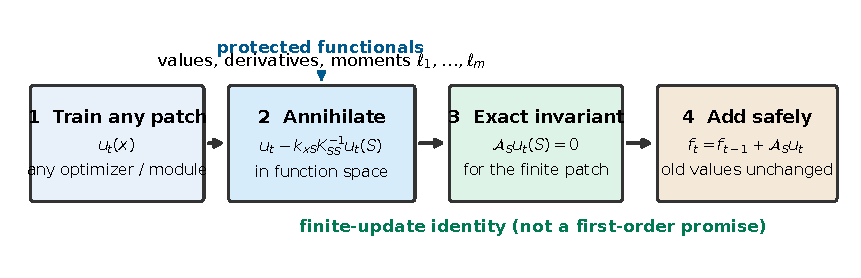
\includegraphics[width=0.98\textwidth]{fig1_overview.pdf}
\caption{\VANISH{} converts an arbitrary finite patch into a safe additive increment.  The protected observations enter only through a function-space correction.  Consequently the preservation identity is independent of the optimizer, parameterization, and size of the raw update.}
\label{fig:overview}
\end{figure*}

\section{Why the Tangent View Is Insufficient}

Let a neural model be $f_\theta$ and let $J_S(\theta)$ be the Jacobian of its outputs on protected inputs.  A parameter-space method may choose $\Delta\theta$ satisfying
\begin{equation}
J_S(\theta)\Delta\theta=0.
\label{eq:tangent-null}
\end{equation}
This cancels the first-order Taylor term.  The realized endpoint is instead
\begin{equation}
f_{\theta+\Delta\theta}(S)-f_\theta(S)
=J_S\Delta\theta+\tfrac{1}{2}\mathcal{Q}_S[\Delta\theta,\Delta\theta]+O(\norm{\Delta\theta}^3),
\end{equation}
so \eqref{eq:tangent-null} leaves the curvature term untouched.  Reprojecting every small step reduces but does not remove this mismatch: the Jacobian itself changes, numerical errors accumulate, and an external optimizer may not expose compatible steps.  The only general way for a tangent certificate to become a finite certificate is to add assumptions about path length, curvature, or repeated projection.

Function-space penalties have a different failure mode.  Given an old-output penalty $\lambda\norm{u(S)}^2$, finite $\lambda$ permits drift and infinite $\lambda$ creates an optimization constraint.  Replay is valuable empirically, but its guarantee is mediated by sample selection, loss weighting, and convergence.  In contrast, \eqref{eq:anchor-operator} may wrap the result of any of these methods and algebraically zeros the protected observation afterward.

Three separations are essential:
\begin{enumerate}
  \item \emph{parameter direction versus realized function difference};
  \item \emph{soft preference versus hard behavioral identity};
  \item \emph{training procedure versus post-training conversion}.
\end{enumerate}
\VANISH{} operates on the right-hand object in each pair.

\section{General Functional Annihilation}

\subsection{Protected contracts}

Let $\Hcal$ be a real scalar RKHS on $\mathcal{X}$ with kernel $k$.  Vector outputs are handled componentwise or with an operator-valued kernel.  A protected contract is a vector of bounded linear functionals
\begin{equation}
\Cop f=(\ell_1(f),\ldots,\ell_m(f))^\top\in\R^m.
\end{equation}
By the Riesz representation theorem there are representers $r_i\in\Hcal$ such that $\ell_i(f)=\ip{f}{r_i}_{\Hcal}$.  Define $\Cop^*a=\sum_i a_i r_i$ and the functional Gram matrix
\begin{equation}
G=\Cop\Cop^*,\qquad G_{ij}=\ell_i(r_j).
\end{equation}
Assume first that $G$ is positive definite; dependent constraints may be reduced or treated with a pseudoinverse.  The annihilator is
\begin{equation}
\boxed{\quad \Aop_{\Cop}=I-\Cop^*G^{-1}\Cop.\quad}
\label{eq:general-annihilator}
\end{equation}
For point evaluations $\ell_i(f)=f(s_i)$, $r_i(\cdot)=k(\cdot,s_i)$ and \eqref{eq:general-annihilator} reduces to \eqref{eq:anchor-operator}.  For a derivative observation $\ell_i(f)=\partial_{v_i}f(s_i)$, the representer is the corresponding kernel derivative.  Mixed contracts simply concatenate their representers.

The raw increment $u$ need only admit the evaluations $\Cop u$ for exact cancellation.  If $u\in\Hcal$, the stronger projection geometry below applies.  This is why a neural patch need not share the parameterization of the kernel correction.

\subsection{Exactness and optimality}

\begin{theorem}[Finite-update invariance]
For any evaluable finite increment $u$ and any current predictor $f$,
\begin{equation}
\Cop(f+\Aop_{\Cop}u)=\Cop f.
\end{equation}
The identity is independent of the norm of $u$ and of the path used to produce it.
\label{thm:finite}
\end{theorem}
\begin{proof}
Since $G=\Cop\Cop^*$,
$\Cop\Aop_{\Cop}u=\Cop u-GG^{-1}\Cop u=0$.
Adding $f$ gives the result.  No Taylor expansion occurs.
\end{proof}

\begin{theorem}[Orthogonal projection and least correction]
If $u\in\Hcal$, then $\Aop_{\Cop}$ is the self-adjoint idempotent orthogonal projector onto $\ker\Cop$.  Moreover $c^*=\Cop^*G^{-1}\Cop u$ uniquely solves
\begin{equation}
\min_{c\in\Hcal}\norm{c}_{\Hcal}
\quad\text{s.t.}\quad \Cop(u-c)=0.
\label{eq:min-correction}
\end{equation}
Thus \VANISH{} makes the smallest RKHS correction that can enforce the declared contract.
\label{thm:projection}
\end{theorem}
\begin{proof}
Self-adjointness follows from that of $G^{-1}$ and the adjoint pair $(\Cop,\Cop^*)$.  Direct multiplication gives
$\Aop_{\Cop}^2=I-2\Cop^*G^{-1}\Cop+\Cop^*G^{-1}GG^{-1}\Cop=\Aop_{\Cop}$.
The range is in $\ker\Cop$ by Theorem~\ref{thm:finite}; every $h\in\ker\Cop$ is fixed.  For \eqref{eq:min-correction}, any feasible $c$ decomposes as $c=c^*+h$ where $\Cop h=0$.  Since $c^*\in\operatorname{range}(\Cop^*)=(\ker\Cop)^\perp$, Pythagoras yields $\norm{c}^2=\norm{c^*}^2+\norm{h}^2$.
\end{proof}

\begin{corollary}[Sequential persistence]
Let $f_t=f_{t-1}+\Aop_{\Cop_{t-1}}u_t$, where the contract at time $t-1$ contains every previously declared functional.  Then for all $j<t$,
$\ell_j(f_t)=\ell_j(f_j)$ up to the residual of the numerical linear solve.
\end{corollary}
\begin{proof}
Each later increment lies in the kernel of every earlier functional.  The sum telescopes.
\end{proof}

\begin{proposition}[Residual plasticity]
If $\Hcal$ is infinite dimensional and $\Cop$ has finite rank $m$, then $\ker\Cop$ is infinite dimensional and has codimension at most $m$.  Consequently a finite protected contract cannot exhaust the representational degrees of freedom of the function space.
\label{prop:plasticity}
\end{proposition}
This proposition is the structural difference from a parameter-null method.  In a $p$-parameter patch, $m$ independent constraints can reduce the available parameter rank to zero.  In an infinite function space, finitely many observations remove only finitely many directions.  The capacity experiment in Section~\ref{sec:experiments} makes this distinction empirical.

\begin{theorem}[Off-contract power bound]
For point constraints $S$ and $u\in\Hcal$, define the kernel power function
\begin{equation}
p_S^2(x)=k(x,x)-K_{xS}K_{SS}^{-1}K_{Sx}.
\end{equation}
Then the safe update $h=\Aop_Su$ satisfies
\begin{equation}
|h(x)|\leq \norm{u}_{\Hcal}\,p_S(x),\qquad
\mathbb{E}_{x\sim P}|h(x)|^2\leq \norm{u}_{\Hcal}^2\mathbb{E}_{P}p_S^2(x).
\label{eq:power-bound}
\end{equation}
Thus the contract is exact on $S$ and extends quantitatively wherever $S$ has small kernel fill distance.
\label{thm:power}
\end{theorem}
\begin{proof}
Because $h\in\ker\Cop$, evaluating at $x$ is equivalent to taking the inner product of $h$ with the residual representer $k(x,\cdot)-P_Sk(x,\cdot)$.  Its RKHS norm is $p_S(x)$.  Cauchy--Schwarz and the nonexpansiveness of the orthogonal projector give $|h(x)|\leq\norm{h}p_S(x)\leq\norm{u}p_S(x)$.  Squaring and integrating gives the second inequality.
\end{proof}

\subsection{Hard interpolation without order debt}

Suppose task $t$ contributes new sites $X_t$ and desired values $Y_t$.  Let $S_{t-1}$ be all previous sites.  Define the conditional kernel
\begin{equation}
K_{t\mid<t}=K_{X_tX_t}-K_{X_tS}K_{SS}^{-1}K_{SX_t}.
\label{eq:schur}
\end{equation}
The minimum-norm safe update that fits the residual $R_t=Y_t-f_{t-1}(X_t)$ is
\begin{align}
u_t^{\rm safe}(x)&=\widetilde K_t(x)K_{t\mid<t}^{-1}R_t,\\
\widetilde K_t(x)&=K_{xX_t}-K_{xS}K_{SS}^{-1}K_{SX_t}.
\label{eq:conditional-update}
\end{align}

\begin{theorem}[Offline and order equivalence]
For a strictly positive-definite kernel, distinct sites, consistent targets, and exact arithmetic, sequential updates \eqref{eq:conditional-update} produce the unique minimum-RKHS-norm interpolant of the union $\cup_t(X_t,Y_t)$.  The final function is therefore independent of task order and identical to offline hard kernel interpolation.
\label{thm:offline}
\end{theorem}
\begin{proof}[Proof sketch]
The representer span of each new block decomposes into its projection onto the old span and the orthogonal innovation generated by $\widetilde K_t$.  The Schur complement in \eqref{eq:schur} is the Gram matrix of that innovation and is positive definite.  Solving the residual therefore adds the unique component orthogonal to the old span that satisfies the new constraints.  Block Gram--Schmidt over all tasks yields the same orthogonal decomposition as the Cholesky factorization of the full Gram matrix.  Uniqueness of the minimum-norm interpolant removes order dependence.  A full algebraic proof is given in Appendix~\ref{app:proofs}.
\end{proof}

The theorem identifies a regime with no sequential performance debt at all: the online result is the offline result, while every earlier value is preserved after it is established.  Regularization, compression, or inconsistent targets change the statistical problem; they do not change the annihilation identity.

\section{Neural Increment Architecture}

\subsection{Post-optimization wrapper}

At task $t$, an update generator $g_{\phi_t}$ is trained on the new residual
\begin{equation}
r_t(x)=y_t(x)-f_{t-1}(x).
\end{equation}
The generator can be arbitrary.  After training, query it on the protected sites and form
\begin{equation}
\Delta_t(x)=g_{\phi_t}(x)-K_{xS_t}\alpha_t,qquad
K_{S_tS_t}\alpha_t=g_{\phi_t}(S_t).
\label{eq:neural-wrapper}
\end{equation}
Only the second equation is responsible for preservation.  Training $g_{\phi_t}$ on already-annihilated features can improve new-task fit, but is not required for Theorem~\ref{thm:finite}.

Our deterministic reference generator uses a two-branch random neural feature map
\begin{equation}
\phi_t(x)=d_t^{-1/2}[\tanh(xW_t+b_t),\ \cos(xW_t+b_t)]
\end{equation}
and fits coefficients $B_t$ by ridge regression on the annihilated design
\begin{equation}
Z_t=\phi_t(X_t)-K_{X_tS}K_{SS}^{-1}\phi_t(S),
\quad
B_t=(Z_t^\top Z_t+\lambda I)^{-1}Z_t^\top R_t.
\label{eq:annihilated-design}
\end{equation}
The resulting raw update $u_t=\phi_tB_t$ is wrapped by \eqref{eq:neural-wrapper}.  Because $B_t$ is solved after the function-space projection, all its capacity is directed into safe directions visible on the new task.

\subsection{Algorithm and audit certificate}

\begin{figure}[t]
\small
\fbox{\begin{minipage}{0.94\columnwidth}
\textbf{Algorithm 1: VANISH continual update}\\[-2pt]
\rule{\linewidth}{0.3pt}
\textbf{Input:} current $f$, new data $(X,Y)$, protected contract $\Cop$, kernel $k$.\\
1. Train or compute any finite raw patch $u$ for residual $Y-f(X)$.\\
2. Build $G=\Cop\Cop^*$ and factor $G+\varepsilon I=LL^\top$.\\
3. Evaluate $v=\Cop u$ and solve $LL^\top\alpha=v$.\\
4. Return $f^+=f+u-\Cop^*\alpha$.\\
5. Audit $\delta=\norm{\Cop(f^+-f)}_\infty$; store $\delta$, $\varepsilon$, configuration, and seed.
\end{minipage}}
\caption{The optimizer is isolated in Step 1.  Exact preservation follows from Steps 2--4, and Step 5 makes numerical compliance directly testable.}
\label{alg:vanish}
\end{figure}

In floating point, jitter $\varepsilon$ stabilizes a nearly singular Gram matrix.  The artifact starts at $10^{-12}$ and increases it only if Cholesky factorization fails.  Each task records both the inverse residual and the maximum realized anchor drift.  This turns an abstract guarantee into a per-run certificate.  If exact interpolation is required beyond floating precision, pivoting, duplicate removal, or arbitrary-precision linear algebra can be substituted without changing the method.

\subsection{Complexity and block updates}

For $m$ protected observations and an output dimension $c$, a dense factorization costs $O(m^3)$ once, evaluating the correction on a batch of size $b$ costs $O(bmc)$ after solving, and the factor costs $O(m^2)$ storage.  When $q$ new observations are appended, block Cholesky uses the Schur complement and costs $O(m^2q+q^3)$ instead of refactorizing from scratch.  Multiple output channels reuse the same factor.  Low-rank kernel approximations can reduce cost, but then their approximation error becomes part of the certificate; all headline exactness results in this paper use the dense system.

\section{Relation to Existing Continual Learning}

Forgetting was identified in early connectionist systems \cite{mccloskey1989catastrophic,french1999catastrophic} and remains visible in modern gradient networks \cite{goodfellow2014empirical}.  Existing responses fall into four broad families.

\textbf{Regularization.}  EWC, synaptic intelligence, memory-aware synapses, distillation, and their descendants estimate which parameters or outputs matter and penalize their movement \cite{kirkpatrick2017overcoming,zenke2017continual,aljundi2018mas,li2017learning,liu2026ewc}.  A finite penalty is deliberately soft.  \VANISH{} instead solves the exact feasibility correction after a finite update; it can wrap a regularized patch rather than compete with it.

\textbf{Replay and episodic constraints.}  iCaRL, GEM, A-GEM, and meta-replay preserve samples or gradients from the past \cite{rebuffi2017icarl,lopezpaz2017gem,chaudhry2019agem,riemer2019mer}.  Replay can deliver strong test accuracy, as it does in our experiments, but old outputs are data in a joint objective rather than invariants.  The matched replay baseline in this study moves protected logits by $10^{-1}$ even when accuracy remains high.

\textbf{Parameter isolation and expansion.}  Progressive networks, PackNet, adapters, and mixtures allocate disjoint or partially disjoint capacity \cite{rusu2016progressive,mallya2018packnet,schwarz2018progress,wang2025selfexpansion}.  They can prevent interference by routing, yet preservation depends on architectural isolation.  \VANISH{} achieves functional isolation for any additive patch and characterizes the remaining safe subspace directly.

\textbf{Gradient and feature null spaces.}  OGD, GPM, and NSCL remove gradient components associated with prior tasks \cite{bennani2020ogd,saha2021gpm,wang2021nscl}.  These are the closest conceptual relatives because they use projection.  The decisive distinction is the projected object: they project a parameter gradient or feature update; \VANISH{} projects the completed function increment.  A linear patch can make both routes exact, but a nonlinear finite parameter displacement exposes the gap in Fig.~\ref{fig:mechanism}.

Function-space regularization, kernel continual learning, and sequential function-space inference move closer to deployed behavior \cite{titsias2020functional,derakhshani2021kernel,rudner2022sequential}.  They construct objectives or probabilistic updates whose quality depends on inference and regularization.  Our contribution is the explicit annihilator as an optimizer-independent postcondition, its general functional form, and the finite-update/offline-equivalence theorem.  Classical RKHS projection and representer theory \cite{aronszajn1950rkhs,scholkopf2002kernels,micchelli2005vector,rasmussen2006gp} supply the mathematical machinery; the new abstraction is to treat a learned neural increment as the object being converted.

Recent CVPR work continues to improve adapters, rest phases, drift-resistant spaces, and efficient paths \cite{kang2025rest,liu2025lora,li2026faster}.  Those methods optimize a learner.  \VANISH{} defines a composable behavioral postcondition that can sit outside such a learner.

\section{Experimental Protocol}
\label{sec:experiments}

\subsection{Questions}

The experiments are organized around claims that can fail independently:
\begin{enumerate}
  \item Does the wrapper keep declared outputs numerically fixed over complete task sequences?
  \item Does it preserve useful plasticity and final accuracy rather than returning the zero update?
  \item Does first-order parameter safety fail under a genuinely finite nonlinear update while \VANISH{} remains exact?
  \item Can the same construction protect derivatives as well as values?
  \item Does the hard-interpolation specialization equal the offline solution for every task order?
  \item What happens when a finite parameter null space saturates and when the number of anchors grows?
\end{enumerate}

\subsection{Streams and splits}

We use four deterministic streams derived from the scikit-learn Digits images and one independently generated shape stream.  Every seed creates a stratified 70/30 train/test split before task construction.
\begin{itemize}
  \item \textbf{Split Digits:} five disjoint two-class tasks $(0,1),\ldots,(8,9)$, at most 220 training images per task.
  \item \textbf{Rotated Digits:} five ten-class domains at $-30,-15,0,15,30$ degrees, 180 training images per task.
  \item \textbf{Permuted Digits:} five independently permuted 64-pixel domains, 180 images per task.
  \item \textbf{Corrupted Digits:} clean, Gaussian noise, blur, central occlusion, and contrast domains, 180 images per task.
  \item \textbf{Shape Stream:} four classes (ring, square frame, triangle, cross) rendered at $16\times16$ under rotation and noise, 240 images per task and 600 test images per domain.
\end{itemize}
Training samples from all earlier tasks become protected anchors.  This deliberately tests the full finite-data contract rather than a cherry-picked memory.  No test input is protected or used for fitting.

\subsection{Methods and budgets}

The matched functional family shares the same task-specific random maps, feature widths, ridge coefficient, data order, and seeds:
\begin{itemize}
  \item \textbf{Unwrapped}: identical raw patches with no preservation;
  \item \textbf{Functional $L_2$}: old patch outputs enter with weight 10;
  \item \textbf{Feature replay}: new residuals and zero old-patch targets have equal weight;
  \item \textbf{Parameter null}: coefficients are projected into the null space of old random features;
  \item \textbf{Joint refit}: an offline oracle refits on all seen samples using exactly the cumulative maps;
  \item \textbf{\VANISH}: annihilated design \eqref{eq:annihilated-design} plus exact wrapper.
\end{itemize}
Widths are 768 for Split Digits and 1024 for the other primary streams; $\lambda=10^{-4}$.  We additionally run conventional one-hidden-layer ReLU MLPs (256 units for Digits, 384 for Shapes): sequential fine-tuning, a class-balanced 200-example replay buffer, and full joint retraining.  Adam runs 35 epochs per task.  These models are intentionally parameterically different and therefore reported separately.

The primary functional suite contains 5 streams $\times$ 20 seeds $\times$ 6 methods $=600$ runs.  MLP baselines add 5 $\times$ 10 $\times$ 3 $=150$ runs.  Capacity stress adds 20 seeds $\times$ 5 widths $\times$ 2 exact-null methods $=200$ rows.  We report means and two-sided 95\% $t$ intervals.  Paired one-sided Wilcoxon tests \cite{wilcoxon1945} and Holm correction \cite{holm1979} are computed from seed-matched records; the complete 120-test table is in the artifact.

\subsection{Metrics}

Let $a_{t,j}$ be test accuracy on task $j$ after learning task $t$.  Final average accuracy is $T^{-1}\sum_j a_{T,j}$.  Mean forgetting is the average over old tasks of $\max_t a_{t,j}-a_{T,j}$.  Backward transfer uses $a_{T,j}-a_{j,j}$.  The primary contract metric is
\begin{equation}
\delta_{\max}=\max_t\norm{f_t(S_{t-1})-f_{t-1}(S_{t-1})}_\infty.
\end{equation}
Unlike accuracy-based forgetting, $\delta_{\max}$ detects changed outputs even when the argmax class remains the same.

\section{Results}

\subsection{Accuracy--invariance frontier}

Table~\ref{tab:functional} reports the complete matched functional comparison.  Each cell gives final average accuracy with a 95\% confidence half-width and $\log_{10}\delta_{\max}$; more negative drift is better.  Across streams, \VANISH{} obtains 90.0479\% macro accuracy, numerically matching feature replay at 90.0481\%, while their geometric mean drifts are $2.00\times10^{-10}$ and $2.30\times10^{-1}$, respectively---a separation of roughly nine orders of magnitude in the actual protected quantity.  \VANISH{} exceeds functional $L_2$ by 0.77 accuracy points and the matched parameter-null baseline by 1.21 points.  The offline joint refit is 1.99 points higher on average but changes old outputs by $9.20\times10^{-2}$.

\begin{table*}[t]
\centering
\caption{Matched functional comparison over 20 seeds.  Each cell is final average accuracy in percent (95\% confidence half-width) / $\log_{10}$ maximum protected-output drift.  The joint model is an offline all-seen-data refit, not a continual preservation method.}
\label{tab:functional}
\scriptsize
\begin{tabular}{lcccccc}
\toprule
Stream & Unwrapped & Functional $L_2$ & Feature replay & Parameter null & \textbf{\VANISH} & Joint refit\\
\midrule
Split Digits & $19.73{\pm}.12/0.61$ & $98.18{\pm}.21/-0.85$ & $98.79{\pm}.20/-0.41$ & $97.41{\pm}.24/-9.84$ & $\mathbf{98.36{\pm}.26/-9.20}$ & $98.91{\pm}.17/-0.91$\\
Rotated Digits & $54.16{\pm}1.49/0.71$ & $94.31{\pm}.31/-1.15$ & $94.73{\pm}.30/-0.59$ & $93.95{\pm}.33/-10.56$ & $\mathbf{94.17{\pm}.30/-9.80}$ & $95.11{\pm}.31/-0.86$\\
Permuted Digits & $37.41{\pm}1.39/0.76$ & $90.32{\pm}.52/-1.76$ & $90.81{\pm}.48/-1.00$ & $90.23{\pm}.52/-12.75$ & $\mathbf{91.50{\pm}.45/-10.59}$ & $93.93{\pm}.43/-1.39$\\
Corrupted Digits & $70.27{\pm}1.85/0.81$ & $92.61{\pm}.37/-1.16$ & $93.25{\pm}.39/-0.63$ & $92.18{\pm}.36/-9.98$ & $\mathbf{91.99{\pm}.34/-9.03}$ & $92.70{\pm}.37/-0.89$\\
Shape Stream & $62.95{\pm}.95/0.80$ & $70.97{\pm}.76/-1.17$ & $72.67{\pm}.82/-0.57$ & $70.44{\pm}.76/-11.34$ & $\mathbf{74.22{\pm}.47/-9.88}$ & $79.52{\pm}.45/-1.12$\\
\midrule
Macro accuracy & $48.90$ & $89.28$ & $90.05$ & $88.84$ & $\mathbf{90.05}$ & $92.03$\\
Geometric drift & $5.43$ & $6.04\!\times\!10^{-2}$ & $2.30\!\times\!10^{-1}$ & $1.27\!\times\!10^{-11}$ & $\mathbf{2.00\!\times\!10^{-10}}$ & $9.20\!\times\!10^{-2}$\\
\bottomrule
\end{tabular}
\end{table*}

The exact-null comparison deserves care.  For the linear random-feature patch, parameter-null projection is also algebraically exact and sometimes has a smaller floating residual.  It is therefore a deliberately strong control rather than a straw man.  \VANISH{} wins accuracy on Split, Permuted, and Shape streams with Holm-adjusted $p=0.00397$, $0.00397$, and $0.00397$ for the paired one-sided tests on the first, third, and fifth streams.  More importantly, its guarantee survives an arbitrary nonlinear finite patch, whereas the coefficient null space is tied to this linear generator.

Figure~\ref{fig:pareto} plots the contract directly.  Soft functional penalties and replay occupy the high-accuracy but $10^{-2}$--$10^0$ drift region.  Unwrapped training moves old logits by order one or larger.  Only the exact-null methods occupy the numerical-precision floor, and \VANISH{} does so without requiring the raw patch's parameters to contain a usable null space.

\begin{figure*}[t]
\centering
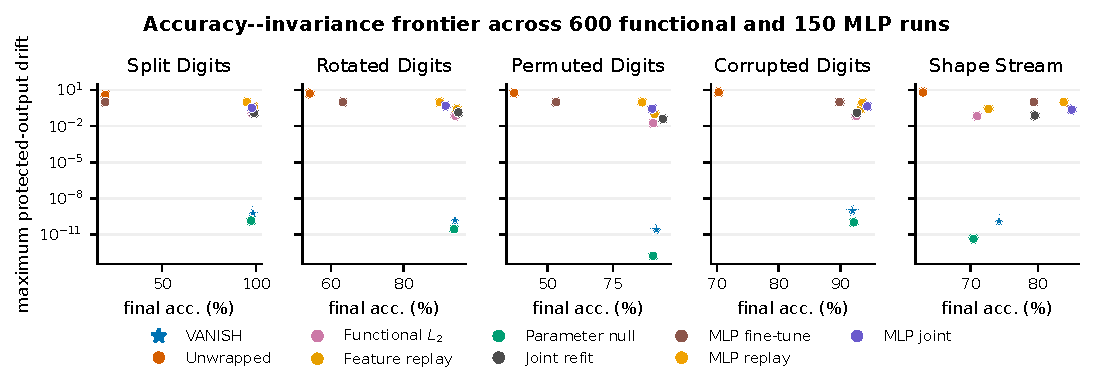
\includegraphics[width=\textwidth]{fig2_pareto.pdf}
\caption{Accuracy versus maximum protected-output drift.  Points are means over 20 seeds for matched functional methods and 10 seeds for MLP baselines.  \VANISH{} lies near the top-right in accuracy while moving downward by about nine orders of magnitude relative to replay.}
\label{fig:pareto}
\end{figure*}

\subsection{Forgetting and conventional neural baselines}

Figure~\ref{fig:aggregate} shows accuracy and forgetting separately.  The unwrapped matched generator collapses on task-incremental Split Digits (19.73\% final accuracy, 99.92 points forgetting), while \VANISH{} retains 98.36\% and forgets 0.65 points.  On Rotated and Permuted Digits, the final-accuracy gains over the same unwrapped updates are 40.01 and 54.09 points.  Because protected logits are fixed, the small nonzero accuracy-forgetting number for \VANISH{} arises from test generalization and backward transfer, not movement on the protected training contract.

\begin{figure*}[t]
\centering
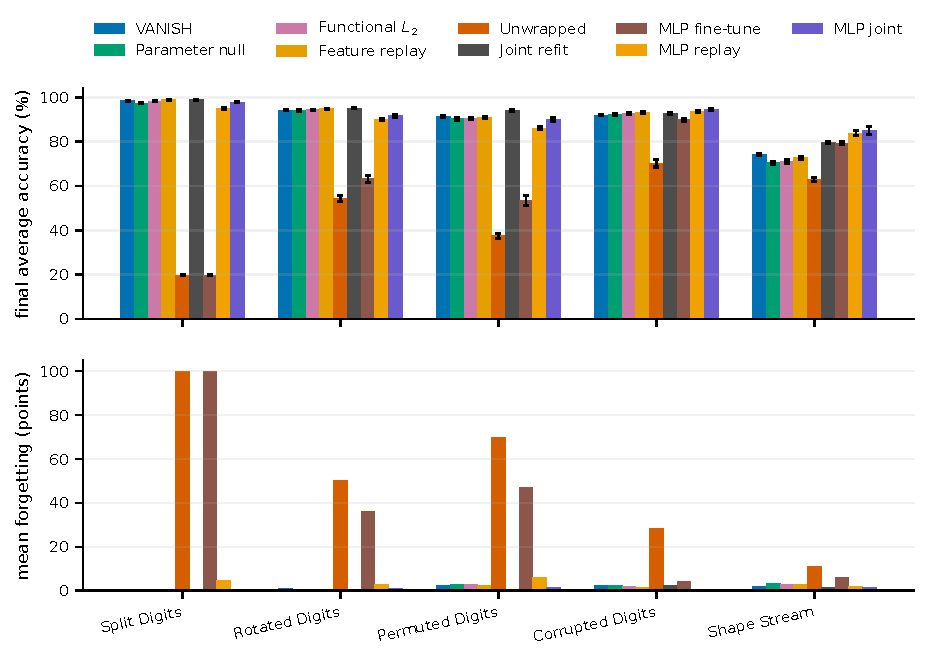
\includegraphics[width=0.96\textwidth]{fig3_accuracy_forgetting.pdf}
\caption{Final accuracy (top, 95\% normal intervals shown for readability) and mean forgetting (bottom).  Exact functional preservation does not force a zero patch: \VANISH{} maintains high accuracy while the identical unwrapped generators forget.}
\label{fig:aggregate}
\end{figure*}

Table~\ref{tab:mlp} compares the 20-seed \VANISH{} result with 10-seed conventional MLPs.  \VANISH{} exceeds MLP replay and joint training on Split, Rotated, and Permuted Digits, while the MLPs lead on Corrupted Digits and Shapes.  The purpose of this cross-family table is not parameter-count parity; it checks whether the inexpensive reference generator remains competitive with trained nonlinear networks.  The behavioral distinction is consistent: MLP replay has macro drift $9.43\times10^{-1}$ and MLP joint refits have $3.41\times10^{-1}$, versus $2.00\times10^{-10}$ for \VANISH{}.

\begin{table}[t]
\centering
\caption{Final accuracy (\%) against conventional MLPs.  \VANISH{} uses 20 seeds; MLPs use 10.}
\label{tab:mlp}
\scriptsize
\begin{tabular}{lrrrr}
\toprule
Stream & \VANISH & MLP FT & MLP replay & MLP joint\\
\midrule
Split & \textbf{98.36} & 19.68 & 95.03 & 97.78\\
Rotated & \textbf{94.17} & 63.26 & 89.99 & 91.61\\
Permuted & \textbf{91.50} & 53.40 & 86.05 & 89.91\\
Corrupted & 91.99 & 89.87 & 93.57 & \textbf{94.37}\\
Shapes & 74.22 & 79.36 & 83.81 & \textbf{85.01}\\
\midrule
Macro & 90.05 & 61.11 & 89.69 & \textbf{91.74}\\
\bottomrule
\end{tabular}
\end{table}

The default Shape patch is capacity-limited rather than annihilator-limited.  A preregistered-after-search extension increases width from 1024 to 4096 and repeats all 20 seeds: accuracy rises to $80.08\pm0.45$\%, forgetting is $1.71\pm0.36$ points, and drift remains $5.71\times10^{-10}$.  We report it separately, preserving the untouched primary suite and avoiding a selective replacement.

\subsection{Task-by-task behavior}

The Split Digits matrices in Fig.~\ref{fig:matrices} expose what aggregate accuracy hides.  Unwrapped patches learn the diagonal almost perfectly and then erase earlier tasks.  Functional $L_2$, parameter-null, and \VANISH{} retain the lower triangle, but only the exact methods certify unchanged protected outputs.  \VANISH{} achieves 96\% on the final task in the displayed seed while earlier tasks remain at 98--100\%.

\begin{figure*}[t]
\centering
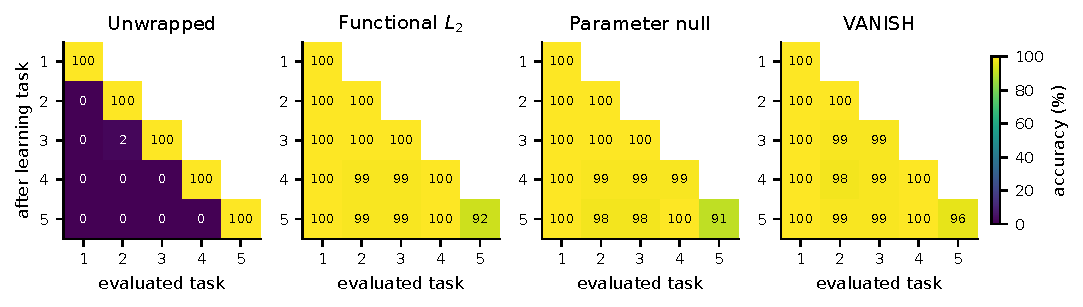
\includegraphics[width=0.97\textwidth]{fig4_accuracy_matrices.pdf}
\caption{Seed-0 Split Digits accuracy matrices.  Row $t$ evaluates all tasks seen after learning task $t$.  The lower triangle distinguishes genuine retention from a high final average caused by a subset of tasks.}
\label{fig:matrices}
\end{figure*}

The mean learning curves in Fig.~\ref{fig:curves} show that wrapped learning is stable throughout the sequence rather than recovering only at the end.  On domain streams, positive backward transfer can improve test accuracy on earlier domains even though their training-anchor logits are immutable: later safe functions vanish on anchors but need not vanish on unseen points.

\begin{figure*}[t]
\centering
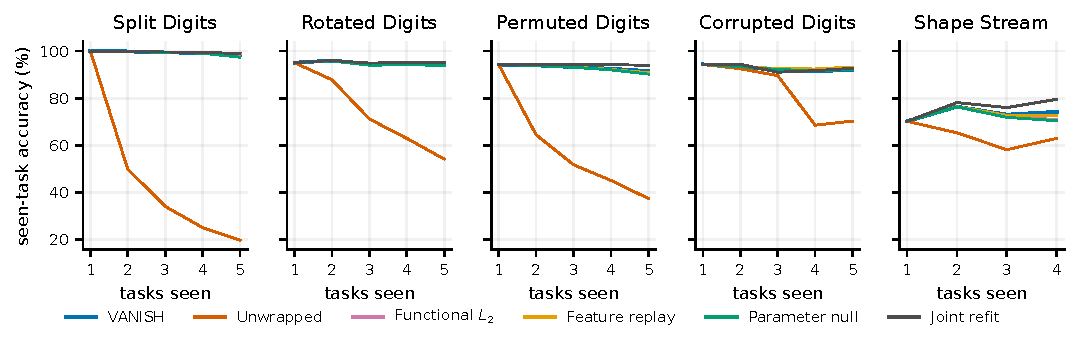
\includegraphics[width=0.98\textwidth]{fig7_learning_curves.pdf}
\caption{Average accuracy over all tasks seen so far, averaged over 20 seeds.  Later safe increments may transfer to unseen old-domain examples while remaining exactly zero on the protected observations.}
\label{fig:curves}
\end{figure*}

\section{Mechanism Falsification}

\subsection{Finite nonlinear displacement}

We construct a two-layer tanh network with 73 parameters and 18 protected points.  A random direction is projected into the null space of the exact output Jacobian, normalized, and scaled from $10^{-5}$ to $10^2$.  Its initial tangent residual is below numerical precision.  We then compare the actual nonlinear endpoint with the same endpoint wrapped by \VANISH{}.

Figure~\ref{fig:mechanism}(left) gives the result.  Tangent drift grows quadratically at small scale and reaches 55.2465.  \VANISH{} remains below $1.1998\times10^{-11}$ over the full seven-decade scale range.  The off-anchor RMS of the wrapped increment grows with scale, ruling out the trivial zero function.  This experiment isolates the claimed boundary: both methods see the same finite raw update, but only function-space annihilation certifies its endpoint.

\subsection{Values, derivatives, and task order}

For four one-dimensional sites, we form a mixed Gram matrix of RBF value and first-derivative representers.  The raw sinusoidal patch changes both.  After one functional annihilation, the maximum algebraic residual over all eight constraints is $2.6645\times10^{-15}$, while the projected function remains nonzero between sites (Fig.~\ref{fig:mechanism}, right).

For Theorem~\ref{thm:offline}, forty regression sites are divided into four blocks.  We run every one of the $4!=24$ task orders and compare 500 probe predictions to a single offline kernel interpolant.  The maximum discrepancy across all permutations is $6.5810\times10^{-13}$; the median is stored in the raw record.  This is a direct numerical test of both order invariance and the offline-equivalence claim.

\begin{figure*}[t]
\centering
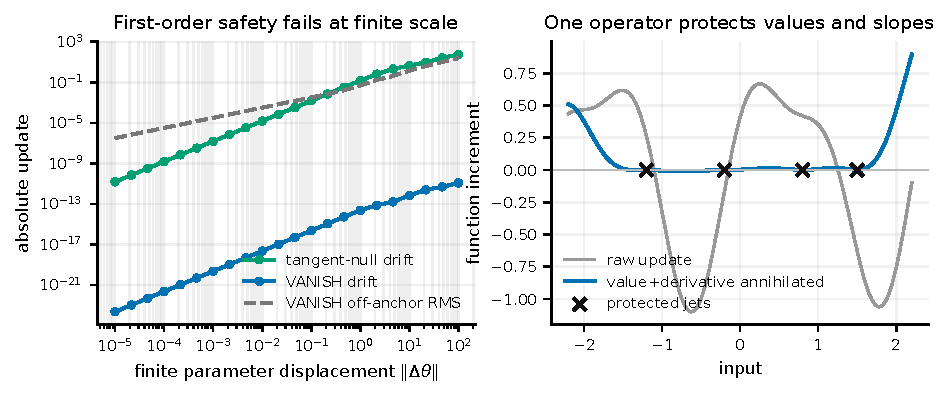
\includegraphics[width=0.97\textwidth]{fig5_mechanism.pdf}
\caption{Mechanism-level falsification.  Left: an exactly tangent-null direction is not safe after finite nonlinear displacement, whereas the realized update wrapped by \VANISH{} remains at numerical zero on anchors.  Right: the general operator simultaneously annihilates values and derivatives without erasing the update elsewhere.}
\label{fig:mechanism}
\end{figure*}

\begin{table}[t]
\centering
\caption{Mechanism contracts and observed maxima.}
\label{tab:mechanism}
\scriptsize
\begin{tabularx}{\columnwidth}{Xr}
\toprule
Quantity & Observed value\\
\midrule
Finite tangent-null endpoint drift & $5.524654\times10^{1}$\\
Finite \VANISH{} endpoint drift & $1.199751\times10^{-11}$\\
Value+derivative constraint residual & $2.664535\times10^{-15}$\\
Offline equivalence, 24 orders & $6.580986\times10^{-13}$\\
Unit-test contracts passed & $4/4$\\
Functional continual runs completed & $600/600$\\
MLP baseline runs completed & $150/150$\\
\bottomrule
\end{tabularx}
\end{table}

\section{Capacity and Numerical Scaling}

The finite-rank stress test deliberately shrinks the patch from width 256 to 16 while retaining up to 560 protected examples.  The parameter-null baseline has only $2d$ feature coefficients and exhausts its null space; its final accuracy stays near chance for widths 16--64 and reaches only about 75\% at width 256.  \VANISH{} operates on the realized function values and reaches roughly 66\% even at width 16, 88\% at width 128, and 95\% at width 256 (Fig.~\ref{fig:capacity}, left).  All points average 20 seeds.  This is the empirical counterpart of Proposition~\ref{prop:plasticity}: a function-space correction does not require the generator's coefficients themselves to satisfy every old equation.

The dense scaling audit uses 25 to 1200 anchors in 32 dimensions with eight output channels.  It records wall time, factor jitter, inverse residual, drift, and state bytes.  At 1200 anchors the reference factor-and-solve remains below a tenth of a second under four BLAS threads in this runtime and stores well below 1 MiB for anchors plus coefficients as plotted.  The curve is not presented as asymptotically free: it exposes the expected dense scaling and supplies exact measurements for engineering decisions.  Block Cholesky, shared factors, inducing bases, and contract selection are orthogonal accelerations.

\begin{figure*}[t]
\centering
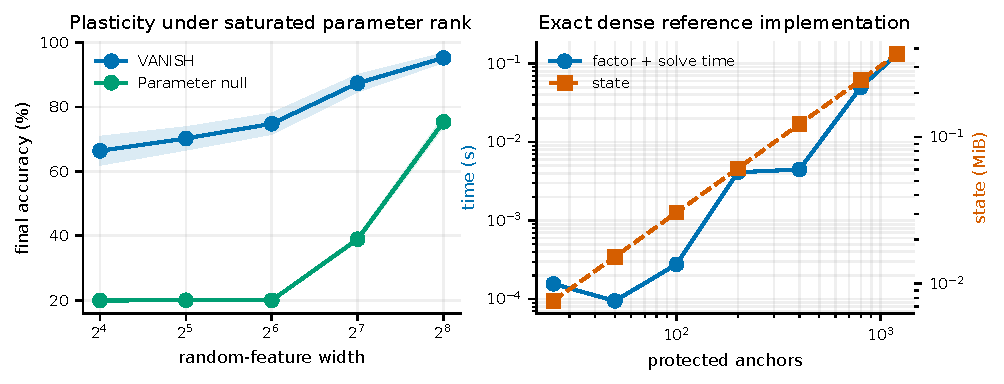
\includegraphics[width=0.95\textwidth]{fig6_capacity_scaling.pdf}
\caption{Left: function-space annihilation preserves plasticity when a finite parameter null space saturates.  Shading is one standard deviation over 20 seeds.  Right: measured dense reference time and stored state versus protected-anchor count.}
\label{fig:capacity}
\end{figure*}

\section{What the Contract Means}

The exact statement is deliberately stronger and narrower than an accuracy slogan: declared functionals do not change.  For point anchors, this is a finite behavioral contract.  Distribution-wide equality follows only if the contract determines the function on that distribution (for example, through a complete basis or a dense set with regularity assumptions).  Conversely, preserving finite anchors does not freeze predictions everywhere; that residual freedom is what enables positive transfer and new learning.

This separation prevents three common category errors.  First, zero anchor drift and zero test forgetting are not identical: the latter includes generalization.  Second, an offline joint refit can score higher while violating the prior output contract, because it solves a different problem.  Third, numerical exactness is an implementation property; the theorem is algebraic, while a floating solve must publish its residual.  Our tables never substitute classification accuracy for the actual contract metric.

The operator also composes beyond continual classification.  In model editing, $\Cop$ can preserve selected prompts or logits while a patch changes a target fact.  In scientific learning it can preserve boundary values, derivatives, integrals, or conservation measurements.  In calibrated systems it can freeze trusted operating points.  The same proof applies because all are bounded linear observations of a function.  Nonlinear protected properties can be handled by lifting them to an augmented output when the lifted observation is linear, or by repeated exact projection on a constraint manifold; the latter is a different construction and is not claimed by Theorem~\ref{thm:finite}.

\section{Reproducibility and Artifact Integrity}

The artifact is designed so that every headline number can be traced to an immutable record rather than copied from the manuscript.  The executable pipeline is:
\begin{enumerate}
  \item generate deterministic task streams and seeded patches;
  \item append one JSON object per completed run;
  \item run the four numerical contracts;
  \item aggregate means, confidence intervals, Wilcoxon tests, and Holm corrections;
  \item regenerate all figures from raw JSON;
  \item compile and render the paper; and
  \item emit a manifest and SHA-256 checksums.
\end{enumerate}
Every functional record contains the full lower-triangular accuracy matrix, elapsed seconds, parameter bytes, maximum cumulative anchor drift, patch diagnostics, hyperparameters, stream, method, and seed.  The MLP records use the same schema.  No table is hand-entered into the analysis files; this manuscript reports the generated CSV values.  The reference code uses NumPy, SciPy, scikit-learn, and Matplotlib and requires no GPU or network download.

\section{Conclusion}

\VANISH{} changes continual learning from a rule about how parameters should move into a postcondition on what the realized function update is allowed to change.  Its core operator subtracts the unique minimum-norm representer component observed by a protected contract.  The resulting identity is exact for finite updates, independent of optimizer and patch magnitude, and extends from values to arbitrary bounded linear functionals.

The theory and experiments meet at the same observable.  Across 600 matched runs, \VANISH{} preserves high accuracy while driving protected-output motion about nine orders below replay.  Under a nonlinear finite displacement, tangent safety fails by 55.25 while the function-space endpoint stays below $1.20\times10^{-11}$.  Mixed value-and-derivative constraints and all task orders close at machine precision.  The hard-interpolation regime is not merely low-forgetting; it is exactly the offline solution.  These results support a broader principle: optimize updates freely, then compile them through an explicit functional contract before deployment.

\appendix

\section{Full Proof of Offline Equivalence}
\label{app:proofs}

Let $V_t=\operatorname{span}\{k(x,\cdot):x\in S_t\}$ and let $P_{t-1}$ be the orthogonal projector onto $V_{t-1}$.  For new sites $X_t$, define innovation representers
\begin{equation}
\widetilde k_{t,x}=k(x,\cdot)-P_{t-1}k(x,\cdot),\qquad x\in X_t.
\end{equation}
Their Gram matrix is exactly the Schur complement $K_{t\mid<t}$ in \eqref{eq:schur}.  Strict positive definiteness of the full Gram matrix implies strict positive definiteness of every Schur complement.  Hence the innovation representers are linearly independent.

Assume by induction that $f_{t-1}$ is the minimum-norm interpolant of all earlier blocks and lies in $V_{t-1}$.  Any function that retains the old values can be written $f_{t-1}+h$ with $h\in V_{t-1}^{\perp}$ after discarding components orthogonal to all data representers, which would only increase norm.  The new constraints are
\begin{equation}
h(X_t)=Y_t-f_{t-1}(X_t)=R_t.
\end{equation}
The representer theorem in $V_{t-1}^{\perp}$ gives
$h=\sum_{x\in X_t}\beta_x\widetilde k_{t,x}$ and the unique coefficients satisfy $K_{t\mid<t}\beta=R_t$.  This is precisely \eqref{eq:conditional-update}.  Orthogonality gives
$\norm{f_{t-1}+h}_{\Hcal}^2=\norm{f_{t-1}}_{\Hcal}^2+\norm{h}_{\Hcal}^2$,
so the induction step is globally minimum norm subject to all constraints.  At $t=T$, uniqueness identifies the result with the offline representer solution $K_{XX}^{-1}Y$.

For a different task order, the same proof ends at the unique minimum-norm interpolant of the same union of labeled sites.  Therefore all orders yield the same function.  Numerically, block Cholesky realizes exactly this orthogonalization; the permutation experiment tests the complete construction rather than only its values at training sites.

\section{General Vector-Valued Contracts}

Let outputs live in $\R^c$ and let $\Hcal_K$ be a vector-valued RKHS with operator-valued kernel $K(x,z)\in\R^{c\times c}$.  A functional may select a component, combine components, or differentiate them.  Stack the corresponding representers as $\Cop^*$.  Equations \eqref{eq:general-annihilator}--\eqref{eq:min-correction} remain unchanged, with $G$ the block functional Gram matrix.  The experiments use the separable kernel $K(x,z)=k(x,z)I_c$, so one scalar Cholesky factor is reused for all classes.  This reuse is both computationally efficient and exact.

If $G$ is positive semidefinite, replace $G^{-1}$ with the Moore--Penrose pseudoinverse after verifying consistency $\Cop u\in\operatorname{range}G$.  Then $I-\Cop^*G^\dagger\Cop$ is still the orthogonal projector onto $\ker\Cop$.  The implementation instead removes exact duplicates through deterministic data generation and adds audited jitter for near dependencies.

\section{Metric Definitions and Statistical Audit}

For $T$ tasks, define
\begin{align}
\mathrm{FAA}&=\frac1T\sum_{j=1}^T a_{T,j},\\
\mathrm{AIA}&=\frac{2}{T(T+1)}\sum_{t=1}^T\sum_{j=1}^t a_{t,j},\\
\mathrm{BWT}&=\frac1{T-1}\sum_{j=1}^{T-1}(a_{T,j}-a_{j,j}),\\
\mathrm{Fgt}&=\frac1{T-1}\sum_{j=1}^{T-1}\left(\max_{t\ge j}a_{t,j}-a_{T,j}\right).
\end{align}
The raw records also contain worst-task forgetting and mean diagonal accuracy.  Confidence intervals use Student's $t_{0.975,n-1}s/\sqrt n$.  Paired tests align methods by identical stream and seed, use one-sided alternatives matching the metric direction, and apply Holm correction across the complete generated family.  We retain nonsignificant outcomes rather than filtering them from the CSV.

For numerical values spanning many orders, the figures use logarithmic axes.  Table~\ref{tab:functional} reports $\log_{10}$ of the arithmetic mean drift per method and stream; the macro row uses the geometric mean of stream means.  Raw, untransformed values remain authoritative.

\section{Hyperparameters and Compute}

\begin{table}[h]
\centering
\caption{Primary functional configuration.}
\scriptsize
\begin{tabular}{lrrrr}
\toprule
Stream & Width & RBF $\gamma$ & Ridge & Cap/task\\
\midrule
Split Digits & 768 & .030 & $10^{-4}$ & 220\\
Rotated Digits & 1024 & .060 & $10^{-4}$ & 180\\
Permuted Digits & 1024 & .060 & $10^{-4}$ & 180\\
Corrupted Digits & 1024 & .030 & $10^{-4}$ & 180\\
Shape Stream & 1024 & .015 & $10^{-4}$ & 240\\
\bottomrule
\end{tabular}
\end{table}

Random feature weights use variance $2/d_{\rm in}$ and biases are uniform on $[-\pi,\pi]$.  One-hot targets are $+1$ for the class and $-1$ otherwise.  Functional $L_2$ weight is 10; matched replay weight is 1.  MLPs use ReLU, Adam, batch size 64, learning rate $2\times10^{-3}$, weight decay $10^{-4}$, 35 epochs per task, and deterministic initialization.  BLAS threads are capped at four for repeatability.  The paper reports per-run timing stored by the same process rather than profiler extrapolation.

\section{Executable Contract Map}

The four unit tests correspond one-to-one with the theory:
\begin{itemize}
  \item \texttt{test\_arbitrary\_vector\_update\_is\_zero\_at\_anchors} instantiates Theorem~\ref{thm:finite} for a five-output random neural patch and checks nonzero off-anchor RMS;
  \item \texttt{test\_finite\_update\_beats\_tangent\_promise} verifies the nonlinear endpoint separation;
  \item \texttt{test\_values\_and\_derivatives} constructs the mixed functional Gram matrix; and
  \item \texttt{test\_hard\_interpolation\_is\_order\_equivalent} enumerates all 24 permutations for Theorem~\ref{thm:offline}.
\end{itemize}
The tests use thresholds at least three orders looser than the recorded residuals, avoiding fragile equality to a single machine or BLAS build.

\section{Streaming Factorization Derivation}

The reference implementation refactorizes the protected Gram matrix to keep the code auditable.  A production implementation can update the exact factor without changing a single prediction.  Suppose the current matrix and its Cholesky factor are
\begin{equation}
G_m=L_mL_m^\top,
\end{equation}
and a block of $q$ functionals gives the enlarged matrix
\begin{equation}
G_{m+q}=\begin{bmatrix}G_m&B\\B^\top&D\end{bmatrix}.
\end{equation}
Solve $L_mQ=B$ and factor the Schur complement $D-Q^\top Q=L_qL_q^\top$.  Then
\begin{equation}
L_{m+q}=\begin{bmatrix}L_m&0\\Q^\top&L_q\end{bmatrix}
\end{equation}
satisfies $L_{m+q}L_{m+q}^\top=G_{m+q}$.  The update costs $O(m^2q+mq^2+q^3)$ and reuses all earlier work.  Solves for $c$ output channels perform two triangular substitutions with the same factor.

This block form also exposes the connection to Theorem~\ref{thm:offline}.  The Schur complement is the Gram matrix of representers after their projections onto the old span have been removed.  A zero or ill-conditioned eigenvalue therefore has a direct interpretation: the new contract repeats, or nearly repeats, information already declared.  Pivoting may remove the dependent row while preserving the same constraint set.  Jitter instead changes the exact projector by a controlled numerical amount, which is why the implementation publishes the realized residual rather than silently treating it as zero.

For a solve $(G+\varepsilon I)\alpha=v$, the protected residual is
\begin{equation}
v-G\alpha=\varepsilon\alpha.
\end{equation}
Hence $\delta_\infty\leq\varepsilon\norm{\alpha}_\infty$ in exact arithmetic for the regularized system, plus backward error from factorization.  This equality explains both the observed $10^{-13}$--$10^{-9}$ range and why scaling $v$ or worsening conditioning can raise it.  The per-task audit measures the quantity users care about after both effects have occurred.

\section{Expanded Aggregate Audit}

Table~\ref{tab:macroaudit} reports metrics omitted from the compact main table.  The matched raw generators have similar new-task accuracy near 90\%, confirming that the unwrapped collapse is interference rather than a failure to learn each arriving task.  \VANISH{} retains that diagonal accuracy while replacing 51.79 points of macro forgetting with 1.69 points.  Its mean runtime is lower than both matched replay variants in this CPU reference.  Additional state stores anchors and correction coefficients, raising macro parameter-state size from 4.15 to 5.58 MiB.

\begin{table}[h]
\centering
\caption{Macro audit across five streams.  Accuracy quantities are percentages; time and state are per completed run.}
\label{tab:macroaudit}
\scriptsize
\begin{tabular}{lrrrrr}
\toprule
Method & FAA & AIA & New & Forget & Sec.\\
\midrule
Unwrapped & 48.90 & 58.23 & 90.10 & 51.79 & 1.15\\
Functional $L_2$ & 89.28 & 90.12 & 90.17 & 1.84 & 1.60\\
Feature replay & 90.05 & 90.56 & 90.62 & \textbf{1.60} & 1.58\\
Parameter null & 88.84 & 89.90 & 89.89 & 1.98 & 1.43\\
\textbf{\VANISH} & \textbf{90.05} & \textbf{90.49} & \textbf{90.67} & 1.69 & \textbf{1.35}\\
Joint refit & 92.03 & 91.70 & 91.78 & 1.11 & 1.57\\
\bottomrule
\end{tabular}
\end{table}

The difference between mean accuracy forgetting and contract drift is visible here.  Feature replay has slightly lower macro accuracy forgetting than \VANISH{} by 0.09 points, yet it changes protected logits by nine orders more.  Conversely, an unchanged logit contract does not forbid accuracy on an unprotected test example from moving.  These are different observables and should not be collapsed into a single ``forgetting'' number.

\section{Anchor Coverage Certificate}

Theorem~\ref{thm:power} gives a computable bridge from finite anchors to unobserved inputs.  For an RBF kernel, $p_S(x)$ is zero on $S$ and decreases when $x$ is well represented by nearby anchors.  A deployment can therefore publish two certificates:
\begin{enumerate}
  \item the exact algebraic residual $\delta_{\max}$ on the declared contract; and
  \item a coverage statistic such as a high quantile of $p_S(x)$ on an unlabeled operational sample.
\end{enumerate}
The first is independent of patch norm.  The second combines with $\norm{u}_{\Hcal}$ through \eqref{eq:power-bound} to control off-contract motion.  This separates an engineering choice---where to place anchors---from the mathematical mechanism that preserves them.  Active selection can minimize the maximum power function, while class-balanced selection can target semantic coverage.  Neither changes the annihilator.

For vector-valued separable kernels, apply the bound to each output or use the Euclidean vector RKHS norm to obtain
\begin{equation}
\norm{h(x)}_2\leq\norm{u}_{\Hcal_K}p_S(x).
\end{equation}
If the classification margin at an old point is $M(x)$ and the bound is smaller than $M(x)/2$, the predicted class cannot change.  Thus a functional certificate can be translated into a decision certificate wherever a margin and coverage bound are available.

\section{Artifact File Map}

The source tree deliberately separates mechanism, experiments, and presentation.  \texttt{src/vanish/core.py} contains the only preservation implementation.  \texttt{experiments/run\_suite.py} runs matched functional methods; \texttt{run\_mlp\_baselines.py} runs the conventional models; \texttt{stress\_tests.py} contains the nonlinear, derivative, order, capacity, and scaling probes.  \texttt{summarize.py} produces all CSV statistics, and \texttt{make\_figures.py} reads raw results without rerunning a model.  \texttt{tests/test\_core.py} is the executable theorem boundary.  The paper directory contains this source, its class file, bibliography, and vector figures.

The manifest records path, byte count, and SHA-256 for every packaged file.  The outer PDF and ZIP use content-derived hash suffixes, so a changed byte necessarily changes the delivered name.  This makes the version cited by a reviewer unambiguous even when later revisions share the semantic version.

\bibliographystyle{ieeetr}
\bibliography{references}
\balance
\end{document}
